\documentclass[11pt,a4paper]{report}
\usepackage[textwidth=37em,vmargin=30mm]{geometry}
\usepackage{calc,xunicode,amsmath,amssymb,paralist,enumitem,tabu,booktabs,datetime2,xeCJK,xeCJKfntef,listings}
\usepackage{tocloft,fancyhdr,tcolorbox,xcolor,graphicx,eso-pic,xltxtra,xelatexemoji}

\newcommand{\envyear}[0]{2025}
\newcommand{\envdatestr}[0]{2025-01-06}
\newcommand{\envfinaldir}[0]{webdb/2025/20250106/final}

\usepackage[hidelinks]{hyperref}
\hypersetup{
    colorlinks=false,
    pdfpagemode=FullScreen,
    pdftitle={Web Digest - \envdatestr}
}

\setlength{\cftbeforechapskip}{10pt}
\renewcommand{\cftchapfont}{\rmfamily\bfseries\large\raggedright}
\setlength{\cftbeforesecskip}{2pt}
\renewcommand{\cftsecfont}{\sffamily\small\raggedright}

\setdefaultleftmargin{2em}{2em}{1em}{1em}{1em}{1em}

\usepackage{xeCJK,xeCJKfntef}
\xeCJKsetup{PunctStyle=plain,RubberPunctSkip=false,CJKglue=\strut\hskip 0pt plus 0.1em minus 0.05em,CJKecglue=\strut\hskip 0.22em plus 0.2em}
\XeTeXlinebreaklocale "zh"
\XeTeXlinebreakskip = 0pt


\setmainfont{Brygada 1918}
\setromanfont{Brygada 1918}
\setsansfont{IBM Plex Sans}
\setmonofont{JetBrains Mono NL}
\setCJKmainfont{Noto Serif CJK SC}
\setCJKromanfont{Noto Serif CJK SC}
\setCJKsansfont{Noto Sans CJK SC}
\setCJKmonofont{Noto Sans CJK SC}

\setlength{\parindent}{0pt}
\setlength{\parskip}{8pt}
\linespread{1.15}

\lstset{
	basicstyle=\ttfamily\footnotesize,
	numbersep=5pt,
	backgroundcolor=\color{black!5},
	showspaces=false,
	showstringspaces=false,
	showtabs=false,
	tabsize=2,
	captionpos=b,
	breaklines=true,
	breakatwhitespace=true,
	breakautoindent=true,
	linewidth=\textwidth
}






\newcommand{\coverpic}[2]{
    % argv: itemurl, authorname
    Cover photo by #2~~(\href{#1}{#1})
}
\newcommand{\makeheader}[0]{
    \begin{titlepage}
        % \newgeometry{hmargin=15mm,tmargin=21mm,bmargin=12mm}
        \begin{center}
            
            \rmfamily\scshape
            \fontspec{BaskervilleF}
            \fontspec{Old Standard}
            \fontsize{59pt}{70pt}\selectfont
            WEB\hfill DIGEST
            
            \vfill
            % \vskip 30pt
            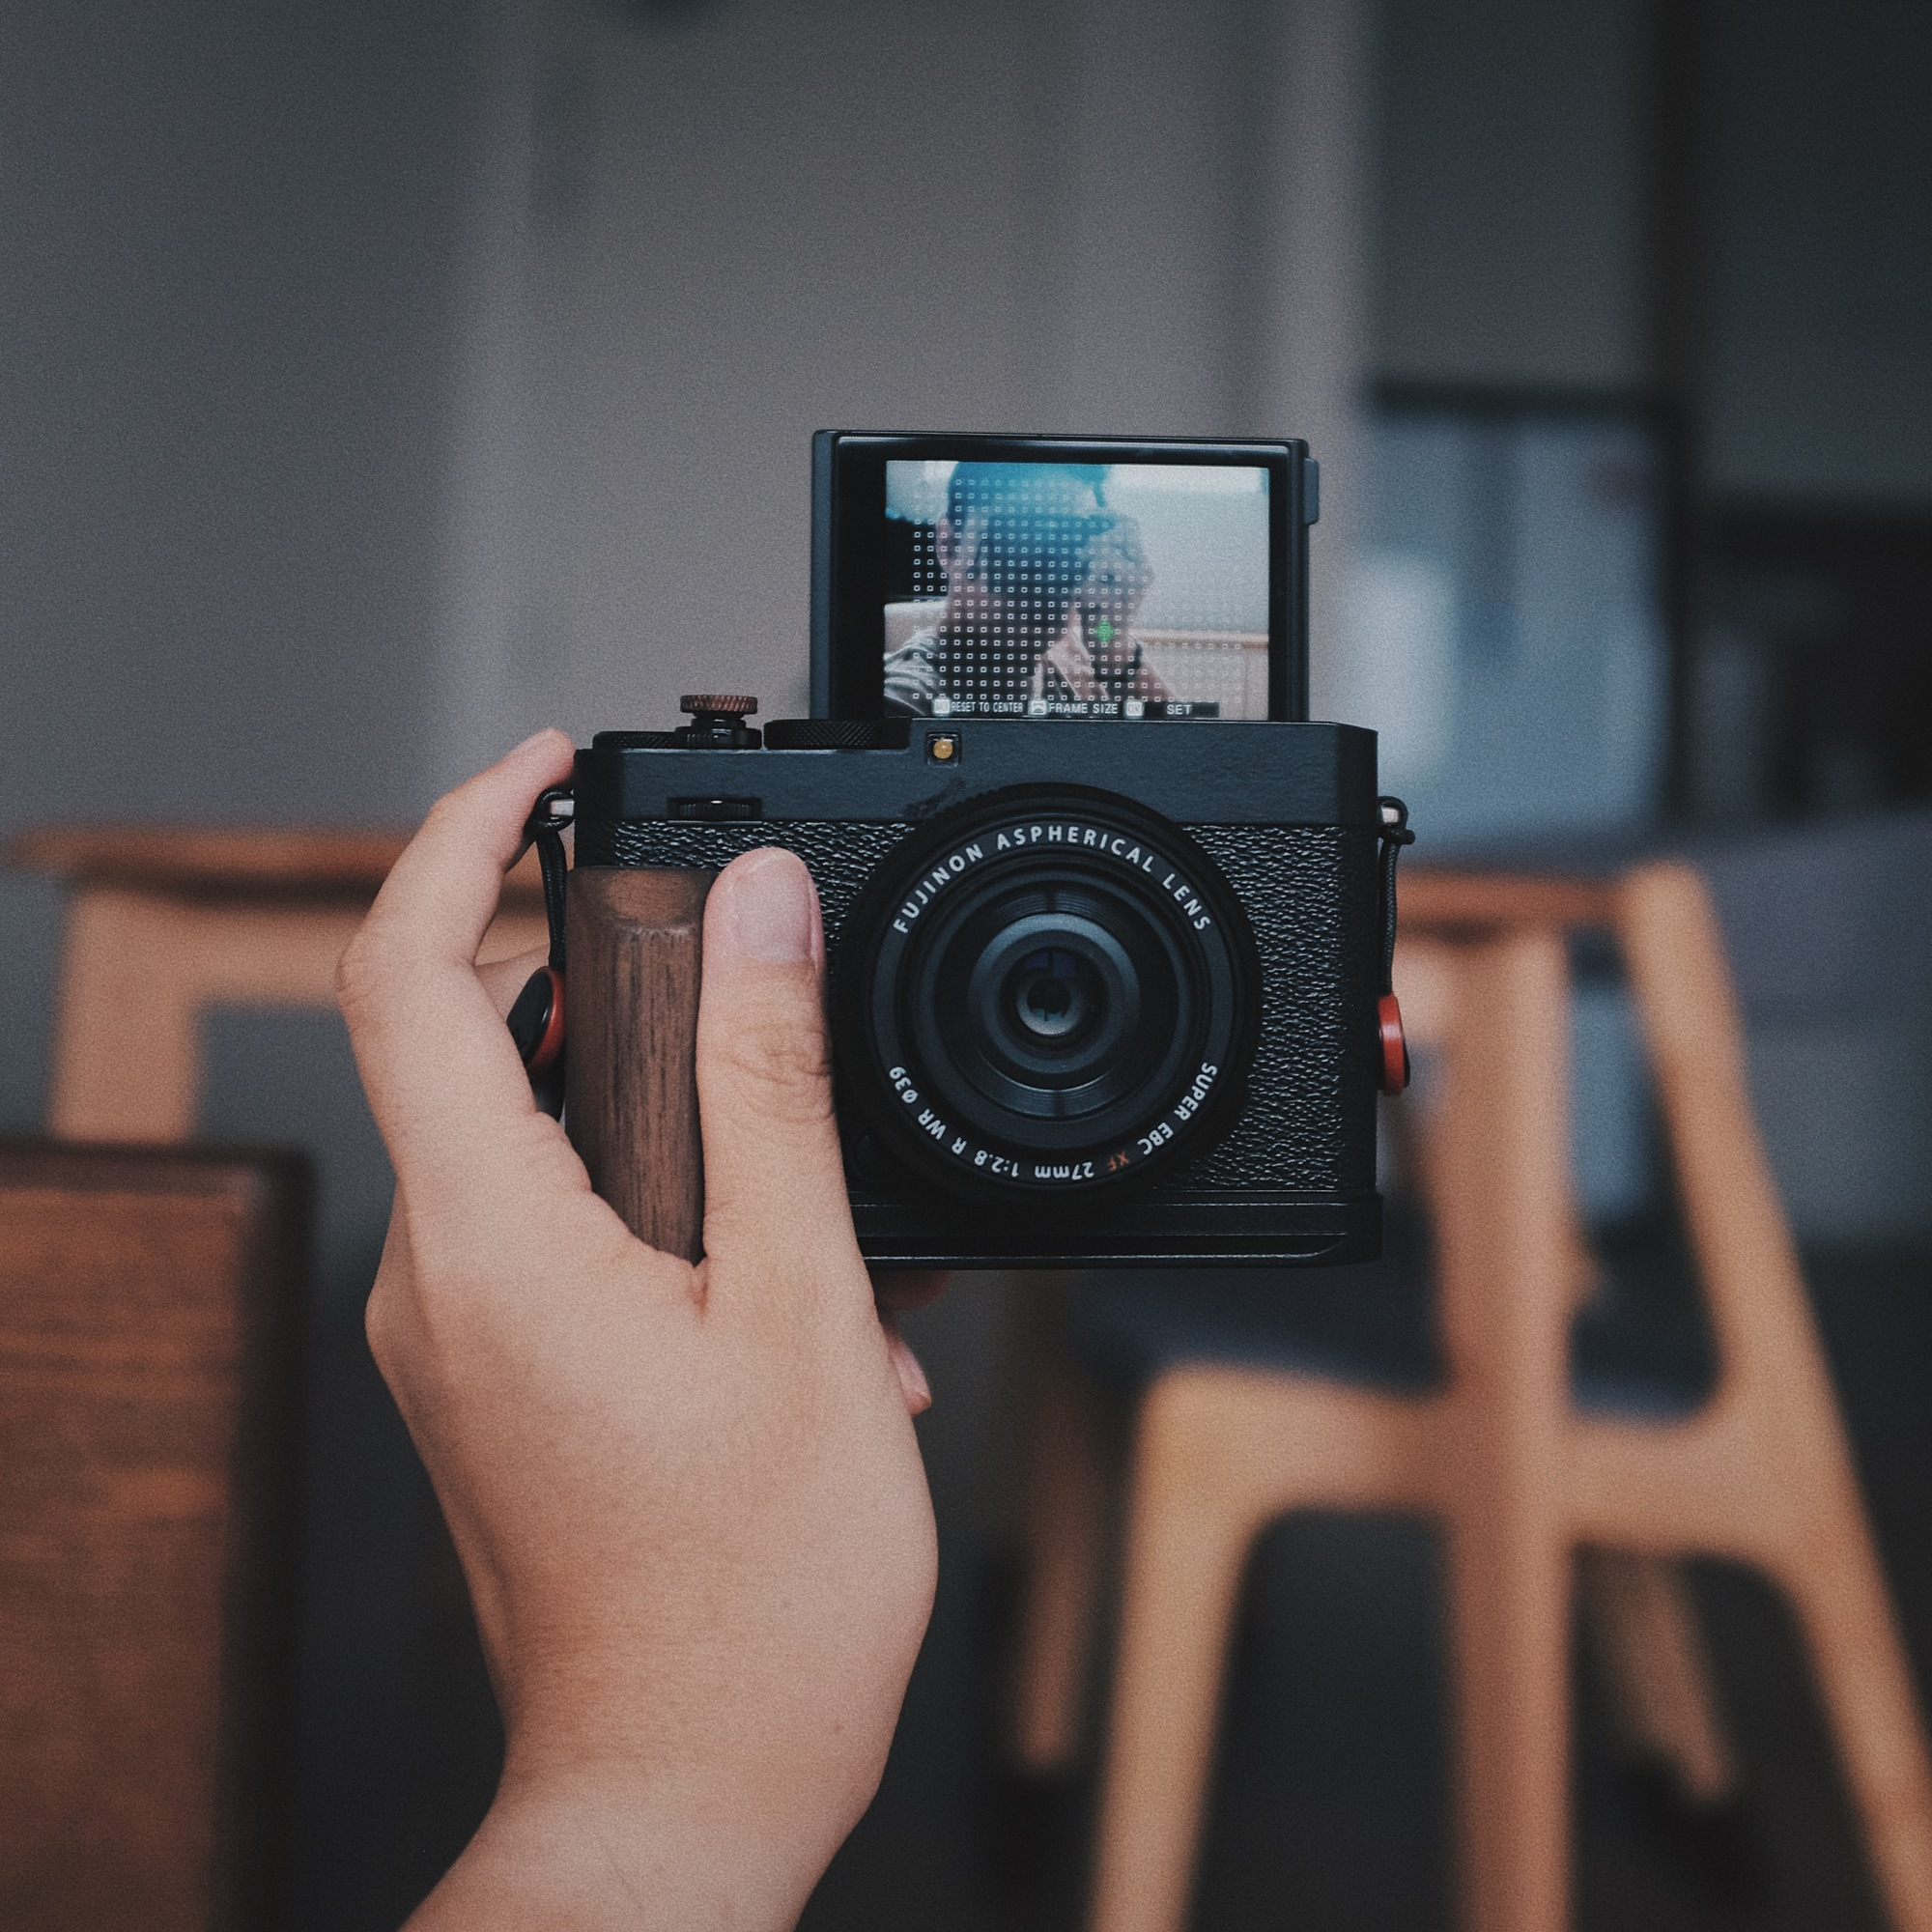
\includegraphics[width=\linewidth]{\envfinaldir/coverpic-prod.jpg}\par
            % \vskip 30pt
            \vfill

            \normalsize\rmfamily\scshape
            \copyright{} The Web Digest Project \hfill\large \envdatestr
        \end{center}
    \end{titlepage}
    % \restoregeometry
}
\newcommand{\simplehref}[1]{%
    \textcolor{blue!80!green}{\href{#1}{#1}}%
}
\renewcommand{\contentsname}{\center\Huge\sffamily\bfseries Contents\par\vskip 20pt}
\newcounter{ipartcounter}
\setcounter{ipartcounter}{0}
\newcommand{\ipart}[1]{
    % \vskip 20pt
    \clearpage
    \stepcounter{ipartcounter}
    \phantomsection
    \addcontentsline{toc}{chapter}{#1}
    % \begin{center}
    %     \Huge
    %     \sffamily\bfseries
    %     #1
    % \end{center}
    % \vskip 20pt plus 7pt
}
\newcounter{ichaptercounter}
\setcounter{ichaptercounter}{0}
\newcommand{\ichapter}[1]{
    % \vskip 20pt
    \clearpage
    \stepcounter{ichaptercounter}
    \phantomsection
    \addcontentsline{toc}{section}{\numberline{\arabic{ichaptercounter}}#1}
    \begin{center}
        \Huge
        \sffamily\bfseries
        #1
    \end{center}
    \vskip 20pt plus 7pt
}
\newcommand{\entrytitlefont}[1]{\subsection*{\raggedright\Large\sffamily\bfseries#1}}
\newcommand{\entryitemGeneric}[2]{
    % argv: title, url
    \parbox{\linewidth}{
        \entrytitlefont{#1}\par\vskip 5pt
        \footnotesize\ttfamily\mdseries
        \simplehref{#2}
    }\vskip 11pt plus 11pt minus 1pt
}
\newcommand{\entryitemGithub}[3]{
    % argv: title, url, desc
    \parbox{\linewidth}{
        \entrytitlefont{#1}\par\vskip 5pt
        \footnotesize\ttfamily\mdseries
        \simplehref{#2}\par\vskip 5pt
        \small\rmfamily\mdseries#3
    }\vskip 11pt plus 11pt minus 1pt
}
\newcommand{\entryitemAp}[3]{
    % argv: title, url, desc
    \parbox{\linewidth}{
        \entrytitlefont{#1}\par\vskip 5pt
        \footnotesize\ttfamily\mdseries
        \simplehref{#2}\par\vskip 5pt
        \small\rmfamily\mdseries#3
    }\vskip 11pt plus 11pt minus 1pt
}
\newcommand{\entryitemHackernews}[3]{
    % argv: title, hnurl, rawurl
    % \parbox{\linewidth}{
    %     \entrytitlefont{#1}\par\vskip 5pt
    %     \footnotesize\ttfamily\mdseries
    %     \simplehref{#3}\par
    %     \textcolor{black!50}{\href{#2}{#2}}
    % }\vskip 11pt plus 11pt minus 1pt
    \begin{minipage}{\linewidth}
            \entrytitlefont{#1}\par\vskip 5pt
            \footnotesize\ttfamily\mdseries
            \simplehref{#3}\par
            \textcolor{black!50}{\href{#2}{#2}}
    \end{minipage}\par\vskip 11pt plus 11pt minus 1pt
}







\begin{document}

\makeheader

\tableofcontents\clearpage




\ipart{Developers}
\ichapter{Hacker News}
\entryitemTwoLinks{Akamai to shut down its CDN operations in China}{https://news.ycombinator.com/item?id=42603585}{https://content.akamai.com/index.php/email/emailWebview?email=NjQyLVNLTi00NDkAAAGWBQgHSPFMp0ow2aF67IAbDOB0c1pNppYjWH8ZCkGxrVi4pDs7pT\_120NiLvARghhVOBbaIJqps\_3Ii2OZlixo3IPjhpR79JsTe-0\&trk=comments\_comments-list\_comment-text}

\entryitemTwoLinks{Ask HN: Politics Blog Cloudflare Subpoena}{https://news.ycombinator.com/item?id=42603292}{https://news.ycombinator.com/item?id=42603292}

\entryitemTwoLinks{Ads chew through half of mobile data}{https://news.ycombinator.com/item?id=42602673}{https://www.nextpit.com/ads-consume-half-of-your-mobile-data}

\entryitemTwoLinks{In my life, I've witnessed three elite salespeople at work}{https://news.ycombinator.com/item?id=42602330}{https://slate.com/life/2024/12/work-jobs-sales-telemarketing-america.html}

\entryitemTwoLinks{A messy experiment that changed how I think about AI code analysis}{https://news.ycombinator.com/item?id=42601847}{https://nmn.gl/blog/ai-senior-developer}

\entryitemTwoLinks{Human study on AI spear phishing campaigns}{https://news.ycombinator.com/item?id=42601681}{https://www.lesswrong.com/posts/GCHyDKfPXa5qsG2cP/human-study-on-ai-spear-phishing-campaigns}

\entryitemTwoLinks{Extracting AI models from mobile apps}{https://news.ycombinator.com/item?id=42601549}{https://altayakkus.substack.com/p/you-wouldnt-download-an-ai}

\entryitemTwoLinks{A story on home server security}{https://news.ycombinator.com/item?id=42601374}{https://raniseth.com/blog/2025-01-04-Home-Server-Security.html}

\entryitemTwoLinks{How NAT Traversal Works (2020)}{https://news.ycombinator.com/item?id=42600846}{https://tailscale.com/blog/how-nat-traversal-works}

\entryitemTwoLinks{Social media distorts perceptions of norms (2024)}{https://news.ycombinator.com/item?id=42600626}{https://osf.io/preprints/psyarxiv/kgcrq}

\entryitemTwoLinks{The funniest thing I ever did – a.k.a. "How To Make \$100K From A Dick Joke."}{https://news.ycombinator.com/item?id=42600595}{https://imgur.com/gallery/KZ4u3c4}

\entryitemTwoLinks{Show HN: Struggle with CSS Flexbox? This Playground Is for You}{https://news.ycombinator.com/item?id=42600586}{https://yoavsbg.github.io/css-flexbox-playground/}

\entryitemTwoLinks{Remote code execution via MIDI messages}{https://news.ycombinator.com/item?id=42600349}{https://psi3.ru/blog/swl01u/}

\entryitemTwoLinks{Back to basics: Why we chose long-polling over websockets}{https://news.ycombinator.com/item?id=42600276}{https://www.inferable.ai/blog/posts/postgres-nodejs-longpolling.mdx}

\entryitemTwoLinks{Hacker gains access to the RP2350 OTP secret by glitching the RISC-V cores}{https://news.ycombinator.com/item?id=42599971}{https://www.tomshardware.com/raspberry-pi/it-looks-like-the-raspberry-pi-rp2350-hacking-challenge-has-been-beaten-hacker-gains-access-to-the-otp-secret-by-glitching-the-risc-v-cores-to-enable-debugging}

\entryitemTwoLinks{Guten: A Tiny Newspaper Printer}{https://news.ycombinator.com/item?id=42599599}{https://amanvir.com/guten}

\entryitemTwoLinks{Researchers design wearable tech that can sense glucose levels more accurately}{https://news.ycombinator.com/item?id=42599189}{https://uwaterloo.ca/news/media/no-more-needles-tracking-blood-sugar-your-wrist}

\entryitemTwoLinks{No-hole surgery: no keyhole, yet surgeons can now still operate under your skin (2023)}{https://news.ycombinator.com/item?id=42599142}{https://www.nibib.nih.gov/news-events/newsroom/getting-under-your-skin-3d-printing-technique-builds-structures-through-tissues}

\entryitemTwoLinks{Web page annoyances that I don't inflict on you}{https://news.ycombinator.com/item?id=42599102}{http://rachelbythebay.com/w/2025/01/04/cruft/}

\entryitemTwoLinks{Nearly half Dell's US workforce has rejected RTO. Rather WFH than get promoted (2024)}{https://news.ycombinator.com/item?id=42598722}{https://www.msn.com/en-us/money/companies/nearly-half-of-dell-s-full-time-workforce-in-the-u-s-has-rejected-returning-to-the-office-they-d-rather-work-from-home-than-get-promoted/ar-BB1oBygb}\ichapter{Phoronix}
\entryitemGeneric{\hskip 0pt{}Linux 6.13-rc6 Released Following A Fairly Quiet Week}{https://www.phoronix.com/news/Linux-6.13-rc6-Released}

\entryitemGeneric{\hskip 0pt{}Xubuntu 25.04 Preparing Xfce 4.20 Desktop Upgrade}{https://www.phoronix.com/news/Xubuntu-25.04-Xfce-4.20}

\entryitemGeneric{\hskip 0pt{}ChromeOS UCSI Driver Queued Ahead Of Linux 6.14 Cycle}{https://www.phoronix.com/news/Linux-6.14-ChromeOS-UCSI}

\entryitemGeneric{\hskip 0pt{}Phoronix Forums Upgrade - Helping To Improve Site Responsiveness}{https://www.phoronix.com/news/Phoronix-Forums-VB6-Upgrade}

\entryitemGeneric{\hskip 0pt{}Loongson Introducing An EDAC Driver For LoongArch + ECC Memory Systems}{https://www.phoronix.com/news/LoongArch-ECC-EDAC-Driver}

\entryitemGeneric{\hskip 0pt{}Serpent OS Demonstrates Working Offline Rollbacks With Its Package Manager}{https://www.phoronix.com/news/Serpent-OS-Offline-Rollbacks}

\entryitemGeneric{\hskip 0pt{}Marvell Begins Working On Linux Support For Their Next-Gen Octeon "CN20K" DPU}{https://www.phoronix.com/news/Marvell-CN20K-Octeon-Linux}

\entryitemGeneric{\hskip 0pt{}Rusticl OpenCL Driver Nearing Cross-Vendor Shared Virtual Memory Support}{https://www.phoronix.com/news/Rusticl-Cross-Vendor-SVM}

\entryitemGeneric{\hskip 0pt{}GNOME Now Has Refine As An Alternative To GNOME Tweaks, Phosh 0.44 Released}{https://www.phoronix.com/news/GNOME-Starts-2025}


\ipart{Developers~~~~(zh-Hans)}
\ichapter{Solidot}
\entryitemGeneric{\hskip 0pt{}RISC-V 笔记本电脑即将走入生活}{https://www.solidot.org/story?sid=80239}

\entryitemGeneric{\hskip 0pt{}美国卫生局局长呼吁为酒加入致癌警告}{https://www.solidot.org/story?sid=80238}

\entryitemGeneric{\hskip 0pt{}黑客通过钓鱼攻击入侵数十个 Chrome 扩展植入后门}{https://www.solidot.org/story?sid=80237}

\entryitemGeneric{\hskip 0pt{}国补将扩大到手机、平板和智能手表等设备}{https://www.solidot.org/story?sid=80236}

\entryitemGeneric{\hskip 0pt{}Windows 10 仍然占据了最大的市场份额}{https://www.solidot.org/story?sid=80235}

\entryitemGeneric{\hskip 0pt{}2024 年挪威销售的九成汽车是纯电}{https://www.solidot.org/story?sid=80234}

\entryitemGeneric{\hskip 0pt{}美国商务部表示考虑限制或禁止中国制造的无人机}{https://www.solidot.org/story?sid=80233}

\entryitemGeneric{\hskip 0pt{}英国 2024 年可再生能源占了电力供应的 45\%}{https://www.solidot.org/story?sid=80232}

\entryitemGeneric{\hskip 0pt{}中国二氧化硫排放量过去 15 年减少了三分之二以上}{https://www.solidot.org/story?sid=80231}

\entryitemGeneric{\hskip 0pt{}蝙蝠一夜之间能飞行近 400 公里}{https://www.solidot.org/story?sid=80230}

\entryitemGeneric{\hskip 0pt{}苹果和 Google 在印度的应用商店下架了多款 VPN 应用}{https://www.solidot.org/story?sid=80229}

\entryitemGeneric{\hskip 0pt{}巨鲸能活得 130 岁以上}{https://www.solidot.org/story?sid=80228}

\entryitemGeneric{\hskip 0pt{}全球生育率下滑和宏观经济发展}{https://www.solidot.org/story?sid=80227}

\entryitemGeneric{\hskip 0pt{}特斯拉全球销量首次下降}{https://www.solidot.org/story?sid=80226}

\entryitemGeneric{\hskip 0pt{}埃博拉病毒可能通过触摸皮肤直接传播}{https://www.solidot.org/story?sid=80225}

\entryitemGeneric{\hskip 0pt{}龙芯开发者向内核递交 32 位 LoongArch CPU 架构支持}{https://www.solidot.org/story?sid=80224}

\entryitemGeneric{\hskip 0pt{}气候变化导致加拿大野火加剧}{https://www.solidot.org/story?sid=80223}

\entryitemGeneric{\hskip 0pt{}普京命令俄罗斯加强与中国在 AI 上的合作}{https://www.solidot.org/story?sid=80222}\ichapter{V2EX}
\entryitemGeneric{\hskip 0pt{}[问与答] 一个很长的 v2 分了好几页的帖子怎么导出为一个 word 文件?}{https://www.v2ex.com/t/1102767}

\entryitemGeneric{\hskip 0pt{}[程序员] 尽管到处裁员,程序员仍是人类历史上最好的职业}{https://www.v2ex.com/t/1102766}

\entryitemGeneric{\hskip 0pt{}[RSS] 超能网的 RSS 是否有问题?}{https://www.v2ex.com/t/1102765}

\entryitemGeneric{\hskip 0pt{}[Kubernetes] 花折 - KubeDoor 正式开源:基于 AI 推荐+专家经验的 K8S 负载感知调度与容量管控系统}{https://www.v2ex.com/t/1102763}

\entryitemGeneric{\hskip 0pt{}[游戏] 发现一个有趣的开源工具 Arnis:让现实世界完美复刻进《我的世界》}{https://www.v2ex.com/t/1102762}

\entryitemGeneric{\hskip 0pt{}[分享创造] 红枫云盘发布 v1.0.1 版本,支持文件加密、压缩以及回收站功能}{https://www.v2ex.com/t/1102760}

\entryitemGeneric{\hskip 0pt{}[问与答] 如何使用简单网管交换机使网口打上主网络 vlan 后连通网络}{https://www.v2ex.com/t/1102758}

\entryitemGeneric{\hskip 0pt{}[摄影] 哪里入手一台靠谱二手照相/摄影机啊?有在日本淘过二手机的网友吗?国内线下有推荐的地方吗?}{https://www.v2ex.com/t/1102757}

\entryitemGeneric{\hskip 0pt{}[加密货币] 截至 2024 年,日本的加密货币用户数已超过 800 万,在中心化交易所,日本用户的日均活跃人数约为 35 万。为什么加密货币会在极其厌恶风险的日本普及开?}{https://www.v2ex.com/t/1102756}

\entryitemGeneric{\hskip 0pt{}[Node.js] 求教: pm2 如何配置一个静态服务器}{https://www.v2ex.com/t/1102755}

\entryitemGeneric{\hskip 0pt{}[C\#] C\# 有哪些显著的缺点?}{https://www.v2ex.com/t/1102753}

\entryitemGeneric{\hskip 0pt{}[Apple] 苹果手表要天天充电 有用过安卓手表配 iPhone 吗}{https://www.v2ex.com/t/1102752}

\entryitemGeneric{\hskip 0pt{}[生活] 不早也不晚的 2024 年终总结(好像是第一次写年终总结}{https://www.v2ex.com/t/1102751}

\entryitemGeneric{\hskip 0pt{}[程序员] 2024 年度总结:勇气}{https://www.v2ex.com/t/1102750}

\entryitemGeneric{\hskip 0pt{}[硬件] 海鲜市场洋垃圾扩展坞求推荐}{https://www.v2ex.com/t/1102749}

\entryitemGeneric{\hskip 0pt{}[智能家电] 如何理解海尔智家 App 首页的水质数值}{https://www.v2ex.com/t/1102748}

\entryitemGeneric{\hskip 0pt{}[硬件] 系统经常遇到未响应,怀疑是硬盘问题, HD Tune 测了下,实惨}{https://www.v2ex.com/t/1102747}

\entryitemGeneric{\hskip 0pt{}[分享创造] 用 AI 做了个工具网站: aab 转 apk}{https://www.v2ex.com/t/1102746}

\entryitemGeneric{\hskip 0pt{}[生活] 有大佬在网上买过沙发吗?}{https://www.v2ex.com/t/1102744}

\entryitemGeneric{\hskip 0pt{}[Apple] M4 mini 24 小时不关机耗电多少}{https://www.v2ex.com/t/1102743}

\entryitemGeneric{\hskip 0pt{}[问与答] 红米 4k 显示器 usb-a 口供电疑问}{https://www.v2ex.com/t/1102742}

\entryitemGeneric{\hskip 0pt{}[随想] 不动脑的贴瓷砖结巴}{https://www.v2ex.com/t/1102741}

\entryitemGeneric{\hskip 0pt{}[分享创造] 订阅合并,去重,重命名,可用性检测}{https://www.v2ex.com/t/1102739}

\entryitemGeneric{\hskip 0pt{}[问与答] 最近买了一台电视,寻求电视看 4k 资源的最佳方案?}{https://www.v2ex.com/t/1102738}

\entryitemGeneric{\hskip 0pt{}[职场话题] 我和公司博弈的經歷(學習積攢和使用權力)}{https://www.v2ex.com/t/1102736}

\entryitemGeneric{\hskip 0pt{}[问与答] 请教下 Java 的 volatile 以及一点多线程的疑问}{https://www.v2ex.com/t/1102734}

\entryitemGeneric{\hskip 0pt{}[香港] 周四去香港办卡,中银需要余额 10W+}{https://www.v2ex.com/t/1102733}

\entryitemGeneric{\hskip 0pt{}[程序员] 远程岗位内推}{https://www.v2ex.com/t/1102732}

\entryitemGeneric{\hskip 0pt{}[DNS] 请教一下 AdGurad Home 的 DNS 重写配置问题}{https://www.v2ex.com/t/1102730}

\entryitemGeneric{\hskip 0pt{}[问与答] 会场舞台上,需要一拖四,两个头戴式麦克风,两个手持式麦克风,能推荐一些品牌和型号吗?}{https://www.v2ex.com/t/1102729}

\entryitemGeneric{\hskip 0pt{}[程序员] 在语雀写的笔记越来越多了,但也发现 CPU 使用率也跟着高了。}{https://www.v2ex.com/t/1102728}

\entryitemGeneric{\hskip 0pt{}[分享发现] 想搞个视频号矩阵, 30 个号左右,有什么可行的方法吗?}{https://www.v2ex.com/t/1102727}

\entryitemGeneric{\hskip 0pt{}[问与答] 在普通的 win 笔记本上用 mac mini 是不是只能插 视频采集卡了 ?}{https://www.v2ex.com/t/1102726}

\entryitemGeneric{\hskip 0pt{}[宽带症候群] 请教海外如何以安全的方式回国内局域网?}{https://www.v2ex.com/t/1102725}

\entryitemGeneric{\hskip 0pt{}[问与答] 给蜗牛星际换了个 sata 背板后进不去群晖了}{https://www.v2ex.com/t/1102724}

\entryitemGeneric{\hskip 0pt{}[问与答] 求推荐适合 MacBook Air m3 使用的 4k 显示器,预算 1k-3k}{https://www.v2ex.com/t/1102723}

\entryitemGeneric{\hskip 0pt{}[Windows] Microsoft 已经草台班子到这种程度了吗}{https://www.v2ex.com/t/1102722}

\entryitemGeneric{\hskip 0pt{}[分享发现] 完全用 cursor 写了一个浏览器插件}{https://www.v2ex.com/t/1102721}

\entryitemGeneric{\hskip 0pt{}[VPS] 荷兰月付 0.9 欧 1c1g25g, 10G 口 150T 流量,三网直连,联通快乐机}{https://www.v2ex.com/t/1102720}

\entryitemGeneric{\hskip 0pt{}[宽带症候群] debian 中的 zerotier 升级 1.14.2 后联网困难怎么回事?}{https://www.v2ex.com/t/1102719}

\entryitemGeneric{\hskip 0pt{}[游戏] 请教关于 switch 舞力全开问题}{https://www.v2ex.com/t/1102718}

\entryitemGeneric{\hskip 0pt{}[问与答] Lan8742 芯片 ping 出现丢包现象}{https://www.v2ex.com/t/1102717}

\entryitemGeneric{\hskip 0pt{}[问与答] cavs/avs2/avs3 视频编码,有什么软件剪切时能看见帧类型}{https://www.v2ex.com/t/1102715}

\entryitemGeneric{\hskip 0pt{}[VPS] 合租国内杜甫}{https://www.v2ex.com/t/1102714}

\entryitemGeneric{\hskip 0pt{}[问与答] Google Voice 申请这么难了么?挂美国 IP 绑定美国手机号都不行}{https://www.v2ex.com/t/1102712}

\entryitemGeneric{\hskip 0pt{}[程序员] 看到有人吐槽 cursor,我也忍不住吐槽一下。}{https://www.v2ex.com/t/1102711}

\entryitemGeneric{\hskip 0pt{}[程序员] electron 公证请教}{https://www.v2ex.com/t/1102710}

\entryitemGeneric{\hskip 0pt{}[汽车] 盘点一下 1.2T 卡罗拉最近这一年的花费}{https://www.v2ex.com/t/1102707}

\entryitemGeneric{\hskip 0pt{}[宽带症候群] 漫游香港-移动流量包使用体验}{https://www.v2ex.com/t/1102706}

\entryitemGeneric{\hskip 0pt{}[分享创造] [VilVil] - 您的多平台视频下载助手!}{https://www.v2ex.com/t/1102705}


\ipart{Generic News}
\ichapter{AP News}
\entryitemWithDescription{\hskip 0pt{}A soccer-loving nun from Brazil is now the world's oldest living person at nearly 117}{https://apnews.com/article/9428ea98d6d2acb0e234a4390404990b}{}

\entryitemWithDescription{\hskip 0pt{}`Mufasa' and `Sonic 3' rule first weekend of 2025}{https://apnews.com/article/d6f138a29ebce4fe3a90ea404a4c74fe}{}

\entryitemWithDescription{\hskip 0pt{}A Melania Trump documentary from director Brett Ratner will be released by Amazon}{https://apnews.com/article/fc36fc99e3eff0a18ef8b72335af88f6}{}

\entryitemWithDescription{\hskip 0pt{}Indie filmmaker Jeff Baena, Aubrey Plaza's husband, found dead at Los Angeles home}{https://apnews.com/article/d626ce1923a9802ba0eb2b951fa45c3c}{}

\entryitemWithDescription{\hskip 0pt{}Washington Post cartoonist quits after paper rejects sketch of Bezos bowing to Trump}{https://apnews.com/article/53928aadc4fb4dda8f35fd840b5717ac}{}

\entryitemWithDescription{\hskip 0pt{}1 person killed in large avalanche in western Wyoming backcountry}{https://apnews.com/article/cf957d7904dca41184e10289655eb651}{}

\entryitemWithDescription{\hskip 0pt{}LeBron James breaks Michael Jordan's record for 30-point games with his 563rd}{https://apnews.com/article/3c60a39c5a6e29b5d9ac497b6de6ee5a}{}

\entryitemWithDescription{\hskip 0pt{}Hundreds of animals killed in Dallas shopping center fire}{https://apnews.com/article/2a6b1be8daf2d42065927fbea4030b95}{}

\entryitemWithDescription{\hskip 0pt{}Retired Eagles great Jason Kelce tries his hand as a late-night television show host}{https://apnews.com/article/d1c5ee89cd87d6c5bda36a4d3aa79be4}{}

\entryitemWithDescription{\hskip 0pt{}Japanese woman who was the world's oldest person at 116 has died}{https://apnews.com/article/914ce99c6f90204311251e2274ae56e8}{}

\entryitemWithDescription{\hskip 0pt{}Joe Burrow and the Cincinnati Bengals keep their playoff hopes alive by edging the Steelers 19-17}{https://apnews.com/article/e5ae4c470cc87af14c1a377098c72e2b}{}

\entryitemWithDescription{\hskip 0pt{}Mother and son given lengthy prison terms for their roles in the killings of 8 Ohio family members}{https://apnews.com/article/0ed638df1a9731fb8a35c2561b6d5dff}{}

\entryitemWithDescription{\hskip 0pt{}What to know about Apple's \$95 million settlement of the snooping Siri case}{https://apnews.com/article/3a543c8f31256b03897cdeaca4cd9b3f}{}\ichapter{Reuters}
\entryitemWithDescription{\hskip 0pt{}Man Utd boss Amorim the 'only guy upset' after spirited draw with Liverpool}{https://www.reuters.com/sports/soccer/man-utd-boss-amorim-only-guy-upset-after-spirited-draw-with-liverpool-2025-01-05/}{Manchester United boss Ruben Amorim was delighted with the intensity his side showed in their breathless 2-2 draw with Premier League leaders Liverpool on Sunday, but said his team\textquotesingle s performance left him wanting...}

\entryitemWithDescription{\hskip 0pt{}Anger and tears as Montenegro town commemorates mass shooting victims}{https://www.reuters.com/world/europe/anger-tears-montenegro-town-commemorates-mass-shooting-victims-2025-01-05/}{Thousands of Montenegrins gathered in the town of Cetinje on Sunday to commemorate the 12 victims of a mass shooting last week, with many accusing police of not having done enough to stop the gunman\textquotesingle s...}

\entryitemWithDescription{\hskip 0pt{}Magnitude 6.1 earthquake strikes El Salvador, EMSC says}{https://www.reuters.com/world/americas/magnitude-61-earthquake-strikes-el-salvador-emsc-says-2025-01-05/}{A magnitude 6.1 earthquake struck El Salvador on Sunday, the European Mediterranean Seismological Centre...}

\entryitemWithDescription{\hskip 0pt{}Farmers' convoys head for Paris to restart protest movement}{https://www.reuters.com/world/europe/farmers-convoys-head-paris-restart-protest-movement-2025-01-05/}{Convoys of farmers set off on Sunday to try to block roads around Paris in protest against what they say is unfair competition from overseas and excessive...}

\entryitemWithDescription{\hskip 0pt{}Rebels seize key town in eastern Congo}{https://www.reuters.com/world/africa/rebels-seize-key-town-eastern-congo-2025-01-05/}{Rwanda-backed M23 rebels have seized a strategic eastern town near the provincial capital Goma in Democratic Republic of Congo, local politicians said on...}

\entryitemWithDescription{\hskip 0pt{}Musk turns on UK's Farage and says he should quit as Reform party leader}{https://www.reuters.com/world/uk/musk-says-farage-should-step-down-leader-reform-uk-2025-01-05/}{It was an abrupt withdrawal of...}

\entryitemWithDescription{\hskip 0pt{}Syrian caretaker government to hike public sector salaries by 400\% next month}{https://www.reuters.com/world/middle-east/syrian-caretaker-government-hike-public-sector-salaries-by-400-next-month-2025-01-05/}{Syria\textquotesingle s finance minister said on Sunday the government would hike salaries for many public sector employees by 400\% next month after completing an administrative restructuring of ministries to boost efficiency and...}

\entryitemWithDescription{\hskip 0pt{}Erdogan expects support from Syria in Turkey's battle with PKK}{https://www.reuters.com/world/middle-east/turkey-says-it-neutralised-32-outlawed-pkk-members-syria-2025-01-05/}{Turkish President Tayyip Erdogan said on Sunday that Syria\textquotesingle s new leadership is determined to root out separatists there, as Ankara said its military had "neutralised" 32 members of the outlawed Kurdistan Workers Party, or...}

\entryitemWithDescription{\hskip 0pt{}Mali rebels say army, Russian fighters killed nine civilians in car attack}{https://www.reuters.com/world/africa/mali-rebels-say-army-russian-fighters-killed-nine-civilians-car-attack-2025-01-05/}{Women and children were among the dead in Mali\textquotesingle s Segou...}

\entryitemWithDescription{\hskip 0pt{}Hamas and Israel wrangle over talks as Israeli strikes in Gaza intensify}{https://www.reuters.com/world/middle-east/israeli-strikes-kill-nine-people-gaza-mediators-strive-truce-deal-2025-01-05/}{The weekend death toll reached 102, Palestinian medics...}

\entryitemWithDescription{\hskip 0pt{}Austria heads towards coalition talks led by far right after centrists fail}{https://www.reuters.com/world/europe/austrian-conservatives-hold-crisis-meeting-after-chancellor-quits-2025-01-05/}{Austria headed on Sunday towards coalition talks led by the far-right Freedom Party (FPO) after efforts to form a centrist government without the FPO fell apart and prompted Chancellor Karl Nehammer to...}

\entryitemWithDescription{\hskip 0pt{}Ukraine launches new attack in Kursk region of western Russia}{https://www.reuters.com/world/europe/russian-war-bloggers-report-new-ukrainian-attack-kursk-region-2025-01-05/}{Russian war bloggers indicated that the latest Ukrainian assault had put Moscow\textquotesingle s forces on the...}

\entryitemWithDescription{\hskip 0pt{}Two Palestinians killed by Israeli forces in the West Bank, Palestinian sources say}{https://www.reuters.com/world/middle-east/palestinian-killed-by-israeli-forces-west-bank-palestinian-sources-say-2025-01-05/}{Israeli forces fired on the home of a 37-year-old man in a town south of Jenin, Palestinian media...}\ichapter{联合早报}
\entryitemWithDescription{沈泽玮:台湾冲突阻遏法案只叫不咬?}{https://www.zaobao.com/news/china/story20240918-4758889}{美国众议院9月9日开启了长达一星期的``中国周'',共通过25项主要涉华法案。(法新社) 美国众议院在当地时间9月9日开启了长达一星期的``中国周'',在美国总统和国会选举举行之前,密集表决数十项与中国有关的法案,共通过25项主要涉华法案……}

\entryitemWithDescription{欧盟电动车关税投票倒计时 中国在分歧中寻支持}{https://www.zaobao.com/news/china/story20240917-4758953}{欧盟27个成员国将于9月25日就是否继续对进口自中国的电动汽车额外征税进行最后表决。图为上海港等待装运出口的电动汽车。(彭博社) 欧盟对中国电动汽车加征关税的投票进入倒计时,正在欧洲访问的中国商务部部长王文涛与欧盟多国政府高层就此进行协商,试图在立场分歧的成员国中争取到更多支持。 受访学者研判,欧盟对中国电动汽车加征关税不可避免,但具体的加税方式和幅度仍有一定弹性,这是王文涛此行与各国谈判的重点……}

\entryitemWithDescription{港府今年将举办逾400项国庆活动}{https://www.zaobao.com/news/china/story20240917-4759341}{再过十多天就是中国国庆75周年,香港天星小轮展示``国庆75周年''\,``三天免费搭小轮''等标语迎国庆。(中新社) 再过十多天就是中国国庆75周年,香港特区政府今年将举办逾400项庆祝活动,希望通过一连串活动庆祝国庆,并且弘扬爱国主义教育及刺激消费。 港府星期二(9月17日)召开记者会,介绍各项庆祝国庆活动和特别优惠,涉及出行及吃喝玩乐等领域……}

\entryitemWithDescription{美空军部长:中国大陆军演精密化 为入侵封锁台湾做准备}{https://www.zaobao.com/news/china/story20240917-4759407}{美国空军部长肯德尔星期一(9月16日)在空军暨太空军协会的一场大会上致辞,提到中国对印太地区日益增长的威胁。(取自美国国防部网站) (华盛顿综合讯)美国空军部长肯德尔指,中国大陆军演的规模越来越大,也更加精密化,这是在专门为入侵、封锁台湾做准备。他也称,中国对印太地区的威胁现在已存在……}

\entryitemWithDescription{批准潜在对台备件军售案后 美派巡逻机过航台海}{https://www.zaobao.com/news/china/story20240917-4758770}{台军士兵8月26日在屏东县枋山训练场进行实弹演习时,从M1167 TOW运载车上发射一枚美制TOW-2A线导反坦克导弹。(路透社) (华盛顿/台北/北京综合讯)在批准潜在对台备件军售案之后,美国派遣反潜巡逻机过航台湾海峡,中国人民解放军东部战区则组织战机跟监美机,并誓言``坚决捍卫国家主权''……}

\entryitemWithDescription{李家超:若香港驻美经贸办被关 受害的是美企}{https://www.zaobao.com/news/china/story20240917-4758797}{香港特首李家超星期一(9月17日)警告,如果美国通过法案,导致香港驻美经贸办关闭,受害的是美国企业。图为李家超9月11日在``一带一路''高峰论坛上致辞。(彭博社) (香港综合讯)香港特首李家超警告,如果美国通过法案,导致香港驻美经贸办关闭,受害的是美国企业。 美国众议院上周通过《香港经济贸易办事处认证法案》,如果参议院也表决通过并交由总统签署成法,香港三个驻美国的经贸办可能将被强制关闭……}

\entryitemWithDescription{美国指中国航空工业集团员工企图实施黑客攻击}{https://www.zaobao.com/news/china/story20240917-4757988}{(华盛顿综合讯)中国航空航天巨头中国航空工业集团一名员工被指试图对美国宇航局、美国军方和其他目标展开黑客攻击。 据彭博社报道,美国检察官布坎南星期一(9月16日)在起诉书中,指控中国航空工业集团39岁的工程师吴宋(音译,Song Wu)企图从美国宇航局、空军、陆军和海军,以及联邦航空管理局取得电脑软件和源代码……}

\entryitemWithDescription{【东谈西论】恒大账务造假 普华永道是共犯还是被拖累?}{https://www.zaobao.com/news/china/story20240917-4756452}{因涉及恒大地产审计项目的违法行为,普华永道中国9月13日被中国财政部和证监会处以4.41亿人民币罚款并被令停业六个月, 广州分所被撤销……}

\entryitemWithDescription{戴庆成:香港输入人才计划大检阅}{https://www.zaobao.com/news/china/story20240917-4744978}{香港于2022年底推出高端人才通行证计划。(法新社) 2019年香港反修例风波过后,数以十万计港人移居海外,令香港出现人才荒。港府为了解决这个问题,在过去几年积极引入``新血'',当中以高才通计划最受瞩目,社会上也不时热议其成效。 高才通全称为高端人才通行证计划,于2022年底推出,申请人年收入须达到250万港元(约42万新元)以上,或本科毕业于全球百强大学并满足一定工作年限等……}

\entryitemWithDescription{中美希望稳定双边关系 中小国家可​​​搭建桥梁}{https://www.zaobao.com/news/china/story20240917-4745091}{中美元首去年11月在旧金山会晤后,双方都希望稳定两国关系,我国巡回大使陈庆珠认为,如果中美两国都认为走向战争不符合它们的利益,那么中小国家就可以做点什么,为双方搭建桥梁。 陈庆珠星期一(9月16日)在李光耀公共政策学院的一场研讨会上说,中国与西方的关系面对诸多困难,有中国智库表示,希望新加坡能协助在中美之间建立更多对话,``因为新加坡受美国信任,也在中国有渠道''……}

\entryitemWithDescription{陈庆珠:世界经历了三次``中国冲击'' 中美的主导力之争将继续}{https://www.zaobao.com/news/china/story20240917-4744996}{李光耀公共政策学院``思想之节庆''的一场研讨会,讨论``历史终结时的中国冲击''。左起是我国巡回大使陈庆珠、通商中国主席李奕贤、李光耀公共政策学院国际关系助理教授何莉菁、李光耀公共政策学院院长柯成兴……}

\entryitemWithDescription{上海遭遇75年来最强台风 扰乱民众中秋假期出行}{https://www.zaobao.com/news/china/story20240916-4745224}{台风贝碧嘉星期一(9月16日)登陆上海,维护人员星期一下午在衡山路上处理倒伏的树木。 (新华社) 台风造成上海上万株数目倒伏或折断。图为一棵倒下的大树砸坏一旁的建筑。(法新社) 台风贝碧嘉登陆上海后,黄浦江苏州河口潮位上涨,乌云密布。(中新社) 中国上海市星期一(9月16日)遭遇75年来最强台风``贝碧嘉''登陆,也是上海有记录以来首次有强台风侵袭……}

\entryitemWithDescription{陆男频长驱偷渡台湾在测试边防实力?}{https://www.zaobao.com/news/china/story20240916-4745161}{中国大陆一名王姓男子在中秋节前夕,乘橡皮艇从浙江宁波抵达台湾新北市林口,主动打电话投案,海巡署人员前去接他上岸。(自由時報) 中国大陆一名王姓男子划橡皮艇于上星期六清晨偷渡到台湾,隔天被新北市地方法院裁定羁押禁见。这是6月以来第二起大陆人士偷渡至台湾,此间专家质疑是否为海防破口,并怀疑对岸是否在测试台湾的边防实力……}

\entryitemWithDescription{中美时隔八月举行国防部工作会晤}{https://www.zaobao.com/news/china/story20240916-4745025}{(北京/华盛顿综合讯)中美双方上周末举行国防部工作会晤;美国官员称,美国积极进行美中两军外交活动,不代表美国对有关中国议题的处理方式发生任何改变。 据中国国防部星期天(15日)晚上通报,北京香山论坛结束后,第18次中美国防部工作会晤上星期六至星期天(9月14日至15日)在北京举行……}

\entryitemWithDescription{中国高校今年拟增足球运动本科专业}{https://www.zaobao.com/news/china/story20240916-4744925}{(北京综合讯)为了培养足球专业人才,中国大专学府今年度拟新增足球运动本科专业,以具体落实中国足球改革。 综合人民网和《南方都市报》报道,中国教育部上星期五(9月13日)发布《2024年度普通高等学校本科专业申报材料公示》。根据公示统计,今年度拟新增专业535个,涉及353所高校,其中39所高校新增足球运动专业……}

\entryitemWithDescription{香港23条首案 港男因穿``光时''上衣被定罪}{https://www.zaobao.com/news/china/story20240916-4743439}{(香港综合讯)香港一名无业男子,今年6月因穿印有2019年反修例抗争口号的上衣而被捕。他星期一承认违反煽动意图罪,成为在《维护国家安全条例》(即《香港基本法》第23条)下被定罪的第一人。 综合港媒《星岛日报》和路透社报道,27岁无业男子诸启邦今年6月12日在石门港铁站附近,未能出示身份证供查阅被警方拘捕……}

\entryitemWithDescription{美国务院:中国释放被关押近20年美籍牧师}{https://www.zaobao.com/news/china/story20240916-4744614}{(华盛顿综合电)中国释放被关押近20年的美国籍牧师,显示北京在中美关系的关键时刻展现善意。 综合彭博社、法新社和路透社报道,美国国务院发言人星期天(9月15日)说:``我们欢迎林大卫(音译,David Lin)从中华人民共和国的监狱获释。他已回返美国,这是他近20年来首次与家人见面。'' 林大卫的女儿艾丽斯告诉美国政治新闻网Politico,她的父亲将抵达得克萨斯州的圣安东尼奥……}

\entryitemWithDescription{中国驻泰使馆:近期并未向湄公河下游泄洪}{https://www.zaobao.com/news/china/story20240916-4743917}{(北京讯)泰国西北部的湄公河因洪水泛滥而决堤,中国否认这是中方泄洪所致,并称近来已持续减少云南景洪水电站的出库流量,以助下游地区抗洪。 中国驻泰国大使馆星期日(9月15日)深夜在官方微信公众号发文说,当天又有媒体报道称中国正在向湄公河泄洪,经向中国主管部门核实,使馆再次澄清,为帮助下游地区应对洪灾,中方近来持续稳定和减少景洪水电站出库流量,不可能对下游地区抗洪救灾形成压力……}

\entryitemWithDescription{加入美国储存可靠度评估计划 台湾军方编列预算采购三类型导弹}{https://www.zaobao.com/news/china/story20240916-4743826}{(台北讯)据台媒报道,台湾军方持续向美国采购可简易操作的导弹,预计在2024年、2031年以前获得400枚``标枪''反装甲导弹、2485枚``刺针''人携式防空导弹……}

\entryitemWithDescription{韩咏红:中美分头追逐全球南方}{https://www.zaobao.com/news/china/story20240916-4730719}{9月5日,中国外长王毅(中)同中非合作论坛非方现任共同主席国塞内加尔外长法勒(左)、下任共同主席国刚果外长加科索(右),在北京共同会见中外记者并答问。(路透社) 进入气候宜人的9月,中国接连举行了两场受瞩目的国际会议,一是聚集非洲53国国家元首与政要的中非合作论坛,接着是周末刚闭幕的北京香山论坛。 两场活动的参与者不同,规模也有很大差距……}

\entryitemWithDescription{菲律宾船只撤离中菲争议海域后 将再派船接替}{https://www.zaobao.com/news/china/story20240915-4730494}{这张在9月15日拍摄,并由菲律宾海岸警卫队提供的照片显示,菲律宾海岸警卫队船马格巴努亚号抵达了菲国巴拉望岛的一个港口。菲律宾早前以发现填海活动为由,今年4月派出马格巴努亚号前往萨比纳礁。(法新社/菲律宾海岸警卫队) 菲律宾国家海事委员会星期天(9月15日)发声明称,该国海岸警卫队一艘巡逻舰已离开萨比纳礁争议海域……}

\entryitemWithDescription{台风贝碧嘉直击中国华东 多趟本地与沪杭间航班取消}{https://www.zaobao.com/news/china/story20240915-4730611}{9月15日在上海外滩滨江步道上,一名外籍游客的雨伞被大风吹起。台风贝碧嘉的中心当天下午5时位于上海市东偏南方大约435公里的东海海面上,中心附近最大风力有13级。(中新社) (上海/新加坡综合讯)台风贝碧嘉预计将为中国华东沿海地区带来狂风暴雨,多趟往返新加坡与上海和杭州的航班取消……}






\clearpage
\leavevmode\vfill
\footnotesize

Copyright \copyright{} 2023-2025 Neruthes and other contributors.

This document is published with CC BY-NC-ND 4.0 license.

The entries listed in this newsletter may be copyrighted by their respective creators.

This newsletter is generated by the Web Digest project.

The newsletters are also delivered via Telegram channel \CJKunderline{\href{https://t.me/webdigestchannel}{https://t.me/webdigestchannel}}.\\
RSS feed is available at \CJKunderline{\href{https://webdigest.pages.dev/rss.xml}{https://webdigest.pages.dev/rss.xml}}.

This newsletter is available in PDF at
\CJKunderline{\href{https://webdigest.pages.dev/}{https://webdigest.pages.dev/}}.

The source code being used to generate this newsletter is available at\\
\CJKunderline{\href{https://github.com/neruthes/webdigest}{https://github.com/neruthes/webdigest}}.

This newsletter is also available in
\CJKunderline{\href{http://webdigest.pages.dev/readhtml/\envyear/WebDigest-20250106.html}{HTML}} and
\CJKunderline{\href{https://github.com/neruthes/webdigest/blob/master/markdown/\envyear/WebDigest-20250106.md}{Markdown}}.


\coverpic{https://unsplash.com/photos/a-couple-of-people-standing-in-a-tunnel-n6TQKt2UlaM}{Alice Kotlyarenko}


\end{document}
